% Chapter 2

\chapter{Finite Element Method} % Main chapter title

\label{Chapter2} % For referencing the chapter elsewhere, use \ref{Chapter1} 

%----------------------------------------------------------------------------------------
%----------------------------------------------------------------------------------------

\newtheorem{definition}{Definition}[section]

\section{Introduction: Poisson Problem} \label{sec:poisson_weak_form}
The Poisson equation is the simplest and the most famous elliptic partial differential equation \cite{arbenz2017}.
Considering a Poisson problem posed in a domain $\mathcal{D}$, a bounded subset of $\mathbb{Rd}$, with prescribed boundary conditions, the problem can be defined in its entirety as:
\begin{equation} \label{def_poisson}
    \begin{cases}
        \nabla ^{2}  u = s  & \text{in $\mathcal{D}$}\\
        u = \overline{u}  & \text{on $\mathcal{S}_{u}$}\\
        q = \frac{\partial u}{\partial x} \cdot \boldsymbol{n} = \overline{q} & \text{on $\mathcal{S}_{q}$},
    \end{cases}
\end{equation}
where \emph{u} defines the unknown potential, $\overline{u}$ is the prescribed value of potential on $\mathcal{S}_{u}$ portion of the boundary and $\overline{q}_{q}$ is the prescribed flux on $\mathcal{S}_{q}$
 with $\mathcal{S} = \mathcal{S}_{u} \cup \mathcal{S}_{q}$ being the boundary of the domain $\mathcal{D}$. The source term is denoted as \emph{s}.
 Equation \eqref{def_poisson} is referred to as a boundary value problem. If $\mathcal{S}_{q} = \emptyset$, the problem is referred to as a Dirichlet problem.
 Similarly, if $\mathcal{S}_{u} = \emptyset$, the problem is called a Neumann problem.
 A third possibility exists for when there's both a prescribed flux and a prescribed value of the potential on disjointed subsets of the boundary such that $\mathcal{S} = \mathcal{S}_{q} \cup \mathcal{S}_{u}$.

A sufficiently smooth function \emph{u} satisfying \eqref{def_poisson} is known as a \emph{classical solution} to the boundary value problem \cite{arbenz2017}.
 This puts a strong condition on \emph{u} to be atleast twice differentiable in the domain $\mathcal{D}$.
However, due to discontinuous source functions or a discontinuous domain, the existence of a classical solution might not be possible.
This is not uncommon and necessitates an alternative description of the boundary value problem
 - called the \emph{weak formulation} as it reduces the constraints imposed upon the solution.
To achieve this two functional spaces must be defined. The space of test functions,
\begin{equation} \label{test_space}
    \mathcal{V} = \{
        w \in H^{1}_{0}(\mathcal{D}) \, | \, \, w = 0 \ \text{on $\mathcal{S}_{u}$}
        \}
\end{equation}
and the space of collection of functions known as trial solutions
\begin{equation} \label{solution_space}
    \mathcal{W} = \{
        u \in H^{1}(\mathcal{D}) \, | \,\, u = \overline{u} \ \text{on $\mathcal{S}_{u}$}.
        \}
\end{equation}
%
Based on the weighted residual method, using these test functions and using the product rule on the right hand side, we get
\begin{align*}
    (s, w) := \int_{\mathcal{D}}  w\, s\,\, dv &= \int_{\mathcal{D}} w \, \nabla^{2} u \,dv\\
    &= \int_{\mathcal{D}}[\nabla(w \, \nabla u) - \nabla w \, \nabla u] \,dv.
\end{align*} 
Applying the divergence theorem,
\begin{equation}
    \int_{\mathcal{D}} \nabla(w \, \nabla u) \,dv = \int_{\mathcal{S}} w (\nabla u \cdot \boldsymbol{n}) \,da
\end{equation}
and substituting the result in the previous equation,
\begin{equation} \label{weak_formulation_1}
    -\int_{\mathcal{D}} \nabla w \cdot \nabla u \, \,dv + 
        \int_{\mathcal{S}} w \,(\nabla u \cdot \boldsymbol{n} \,da)  =  \int_{D} w \, s \, \,dv.
\end{equation}
As $w = 0$ on $\mathcal{S}_{u}$ and according to the problem statement and the definition of Neumann boundary conditions, equation
 \eqref{weak_formulation_1} can be written as
\begin{equation} \label{weak_formulation_2}
    - \int_{\mathcal{D}} \nabla w \cdot \nabla u \, \,dv = \int_{\mathcal{D}} w \, s \,\,dv - \int_{\mathcal{S}_{q}} w \, \overline{q} \,\,da.
\end{equation}

\subsection{Function Spaces and Well-Posedness of the Weak Formulation} 
For the equality in \eqref{weak_formulation_2} to make sense, it is no longer necessary for \emph{u} to be twice differentiable. The classical definition of a derivative
 is stated pointwise - thus requiring the function to be defined at all points. For \eqref{def_poisson}, this implies that \emph{u} be $C^{2}$ continuous. The weak derivative involed in the weak formulation is more general and includes functions that
 that are not necessarily $C^{2}$ contininuous throughout the domain. This requires the definition of a function space where it is possible to define a weak derivative.
 This function space is where the \emph{test functions} and \emph{trial solutions} live. This function space is called a \emph{Sobolev space}. 
 Using the space of square integrable functions,
 \begin{equation} \label{square_integrable_space}
    L^{2}(\Omega) = \left\{f: \Omega \to \mathbb{R} : \int_{\Omega} |f|^{2} < \infty \right\},
 \end{equation} 
 the Sobolev spaces for a given $f \in L^{2}(\Omega)$ can be defined as
\begin{equation}\label{sobolev_space}
    H^{1}(\Omega) = \left\{f \in L^{2}(\Omega): \frac{\partial f}{\partial x_{1}}, \frac{\partial f}{\partial x_{2}} \in L^{2}(\Omega)\right\}.
\end{equation}
and,
\begin{equation} \label{hilbert_space}
    H^{1}_{0}(\Omega) = \left\{f \in H^{1}(\Omega): f = 0 \text{ on } \partial \Omega\right\}
\end{equation}
is the special Sobolev space, which is the set of all functions \emph{f} in $H^{1}(\Omega)$ such that $u = 0$ on the boundary of the domain \cite{suli2012}.
 Thus for partial differential equations with a Dirichlet boundary condition, it is natural to look for a test function belonging to $H^{1}_{0}$, 
 and the trial solutions to be a part of $H^{1}$.
If the all the first derivatives on the left hand side of \eqref{weak_formulation_2} are in $L_{2}(\mathcal{D})$,
 $\overline{q} \in L_{2}(\mathcal{S}_{q})$, and $s \in L_{2}(\mathcal{D})$, the equation \eqref{weak_formulation_2} is well posed in the sense of Hadamard \cite{suli2012}.
 Furthermore, there exists a weak solution $u \in H^{1}(\mathcal{D})$ that is also a solution to \eqref{def_poisson} \cite{brenner2002}. 
 According to the Lax-Milgram theorem, the weak solution obtained from the solution of \eqref{weak_formulation_2} is unique \cite{larcher2013}.
 For a thorough mathematical treatment, the reader is referred to \cite{brenner2002}.  
%-----------------------------------------------------------------
%
%
\section{Construction of a Finite Element Space}
Approximation methods can be broadly divided in two categories.
\begin{itemize}
    \item The given function is approximated using linearly independent functions and parameters. This is a
     \emph{non-nodal approximation} and is written as
     \begin{equation}
        u(x) = P_{1}(x) a_{1} + \dots + P_{n}(x) a_{n}, \notag
     \end{equation}
     where $P_{1}, P_{2},\dots, P_{n}$ are linearly independent known functions, 
     and $a_{1}, a_{2},\dots, a_{n}$ are the parameters of the approximation. These parameters generally do not have any physical meaning.
    \item In \emph{nodal approximations} the parameters $a_{i}$, as described above, can be chosen to be the values of the function \emph{u} at \emph{n} different coordinates $x_{i}$. Thus,
    \begin{align*}
        u(x_{1}) &= u_{1} = a_{1}\\
        u(x_{2}) &= u_{2} = a_{2}\\
        u(x_{3}) &= u_{3} = a_{3}\\
        \dots \\
        u(x_{n}) &= u_{n} = a_{n}
    \end{align*}   
    turning the approximation to be, 
    \begin{equation*}
        u(x) = N_{1}(x) a_{1} + N_{2}(x) a_{2} + ... + N_{n}(x) a_{n}
    \end{equation*}
    where $N_{1}, N_{2},\dots, N_{n}$ are called \emph{shape functions} that have the property
    \begin{equation*}
        N_{i}(x_{j}) = \begin{cases}
            0 \text{, if } \, i \neq j\\
            1 \text{, if } \, i = j
        \end{cases}
    \end{equation*}
\end{itemize}
Nodal approximation methods are preferred over non-nodal approximations as non-nodal approximations require
 linearly independent functions that are well defined throughout the domain. For a domain with a complex boundary,
 it makes the fulfilment of boundary conditions difficult and require increased computational power due to the dense system
 of equations required to solve the problem. Nodal approximation methods involve piecewise defined shape functions. While it may be difficult to satisfy the
 completeness and continuity criterias involved, due to the final system of equations being sparse and the local support of shape functions,
 the advantage of drastically reduced computation offsets the negatives. The Finite Element Method provides a formalism for generating discrete algorithms for approximating
 the solutions of differential equations using nodal approximations. 
 Formally, according to \cite{ciarlet1978finite}, 
\begin{definition}
    a Finite Element is a set of triples, $(K, \mathcal{P}, \mathcal{N})$, where
    \begin{itemize}
        \item $K \subseteq \mathbb{R}^{n}$ be a bounded closed set with nonempty interior and piecewise smooth boundary (the element domain),
        \item $\mathcal{P}$ be a finite-dimensional space of functions on K (the space of shape functions) and
        \item $\mathcal{N} = {N_{1}, N_{2},...,N_{n}}$ be a basis for the dual space of $\mathcal{P}$ (the set of nodal variables).
    \end{itemize}
\end{definition}
%
The closed set $K$ defines the element subdomain being used in the calculation. $\mathcal{P}$ delineates the set of
 the shape functions involved in the approximation, and $\mathcal{N}$ is the set of nodal variables i.e. the nodes at
 which the function is approximated. For a linear quadrilateral element $K$, $\mathcal{P}$ can be characterised by saying
 that the overall approximation is continuous and for a linear approximation on the vertices $i, j, k, l$,
 there are only four basis functions, $\left\{\Phi_{i}, \Phi_{2}, \Phi_{3}, \Phi_{4} \right\}$ that are not identically zero.
 This is the Kronecker delta property and can be written as
 \begin{equation}
    \mathcal{N}_{i}(\Phi_{j}) = \delta_{ij}.
 \end{equation}
It is assumed that these conditions ensure the interpolation problem using functions in $\mathcal{P}$ is uniquely solvable.
 For proof, refer to \cite{brenner2002}. The approximation of the variable field that would be the solution to the PDE is the basis of $\mathcal{P}$.
 The construction of a finite element, thus, involves:
 \begin{itemize}
    \item choosing an element domain
    \item choosing a polynomial space of a given degree
    \item choosing the degrees of freedom (number of nodes)
    \item computing the nodal basis of $\mathcal{P}$ with respect to $\mathcal{N}$.
 \end{itemize}

With the derived weak form \eqref{weak_formulation_2}, it is possible to use the finite element method to solve the given problem.
Let the domain $\mathcal{D}$ be discretised into finite elements $\mathcal{D}^{e}$ such that
\begin{equation}\label{discretisation_definition}
    {\mathcal{D}} = \bigcup^{n_{el}}_{e=1} {\mathcal{D}}^{e},
\end{equation}
where $\mathcal{D}^{e} \cap \mathcal{D}^{f} = \emptyset \, \, \text{for } e \neq f$ which implies that these have no overlap.
 Furthermore, these finite elements can only share nodes along common facets in order to preserve the compatibility 
 of the primary variables and the equilibrium within the elements and along the shared facets. 
 
With the discretisation defined, the functional spaces for the shape functions and the trial solutions can be defined, similar to Section
 \ref{sec:poisson_weak_form} as
\begin{align}\label{discretised_spaces}
    \mathcal{V}^{h} = \left\{w \in H^{1}(\mathcal{D})\,\, |\,\, w|_{\mathcal{S}^{e}} \in \mathcal{P}_{m}(\mathcal{D}^{e}) \, \forall \,\, e \text{ and } w = 0 \,\, \text{on } \mathcal{S}_{u}\right\},\\
    \mathcal{W}^{h} = \left\{u \in H^{1}(\mathcal{D})\,\, |\,\, u|_{\mathcal{S}^{e}} \in \mathcal{P}_{m}(\mathcal{D}^{e}) \, \forall \,\, e \text{ and } u = \overline{u} \,\, \text{on } \mathcal{S}_{u}\right\}
\end{align}
%
The position vectors can be approximated as
\begin{equation} \label{pos_vectors}
    \boldsymbol{x} \approx \boldsymbol{x}^{h} = \mathbf{N}^{e}\mathbf{x}^{e}, \,\,\, \boldsymbol{x}^{h} \in \mathcal{D}^{e} \subset \mathcal{S}^{h},
\end{equation}
where
\begin{equation} \label{shape_functions}
    \mathbf{N}^{e} = [N_{1}\boldsymbol{1}, N_{2}\boldsymbol{1},...,N_{n^{e}_{n}}\boldsymbol{1}],
\end{equation}
where $\mathbf{N}^{e}$ denotes the $(d \, \times \, d*n^{e}_{n})$ array, $n^{e}_{n}$ denotes the number of element nodes, \emph{d} number of degrees of freedom
 for a given node, $N_{i}$ the nodal shape functions, and $\boldsymbol{1}$ is the identity matrix. For a potential function, the discretisation can be given as
 \begin{equation} \label{discretisation_def}
    u(\boldsymbol{x}) \approx u^{h}(\boldsymbol{x}) = \sum^{n_{en}}_{k=1} N^{e}_{k} u^{e}_{k} = \mathbf{N}^{e} \mathbf{u}^{e}.
 \end{equation}
In the current case, \emph{u} is a scalar field such that the degree of freedom $d = 1$.
 Using Galerkin formulation, the arbitrary test functions can be defined as
\begin{equation}
    w^{h} \in \mathcal{V}^{h} := \underset{{e = 1,...,n_{el}}}{\mathrm{span}}\{\mathbf{N}^{e}\}.
\end{equation}
%
Using the above definitions, it is possible to write the discretised system of equations as 
\begin{equation}\label{discretised_poisson}
    \underbrace{-\sum^{n_{el}}_{e=1} \int_{\mathcal{D}^{e}} \nabla \, N_{a} \cdot \nabla \, N_{b} \, dv}_{\boldsymbol{\mathrm{K}}} \underbrace{u_{b}^{e}}_{\boldsymbol{\mathrm{u}}} = 
    \underbrace{\sum^{n_{el}}_{e=1} \int_{\mathcal{D}^{e}} N_{b}\, s \,dv - \sum^{n^{b}_{el}}_{e=1} \int_{\mathcal{S}^{e}_{q}} N_{b} \,\overline{q} \,da}_{\boldsymbol{\mathrm{f}}}  ,
\end{equation}
where $n^{b}_{el}$ denotes the number of elements laying on the boundary where the Neumann boundary conditions are prescribed. The system of thus discretised linear equations required to solve the
 model problem \eqref{def_poisson} can be written in a compact form as
 \begin{equation}\label{FEM}
    \boldsymbol{\mathrm{Ku}} = \boldsymbol{\mathrm{f}}, 
 \end{equation}
where the elemental contributions are defined as,
\begin{gather}\label{K_and_f}
    \boldsymbol{\mathrm{K}}^{e}_{ab} = -\int_{\mathcal{D}^{e}} \nabla N_a \cdot \nabla N_b \, dv,\\
    \boldsymbol{\mathrm{f}}^{e}_{b} = \int_{\mathcal{D}^{e}} N_b s \,dv - \int_{\mathcal{S}^{e}_{q}} N_{b} \,\overline{q} \,da.
\end{gather}

\section{Isoparametric Elements} \label{sec:isoparametric_theory}
The Finite Element Method consists of discretisation at two levels - the domain of the problem is discretised into finite elements, and the field of primary variables
 is approximated using interpolation functions. When dealing with complex domains, in order to decrease the geometrical discretisation error, it becomes necessary to
 use 'irregular' elements - elements that necessarily would not have straight line edges or faces.
 However, it may often not be possible to define interpolations that result in \emph{conforming approximations} over these irregular elements. 
To ensure conforming approximations basis functions can be defined over a reference element. For a reference quadrilateral,
 $\xi \in [-1,1]$ and $\eta \in [-1, 1]$, the basis functions can be constructed using Lagrangian polynomials of order $n$.
 For a node characterised by its row $i$ and column $j$, the corresponding shape function can be given by,
 \begin{equation}
    N_{ij} = l^{n}_{i}(\xi) \, l^{n}_{j}(\eta), \text{ where } l^{n}_{k}(\xi_{i}) = \prod^{n}_{k = 1, k \neq i} \frac{\xi_{k} - \xi}{\xi_{k} - \xi_{i}} = \begin{cases} 
        1, i = k \\
        0, i \neq k
    \end{cases}
\end{equation} 
These functions are then mapped from the reference element to any general quadrilaateral with vertex coordinates, $(x_{q}, y_{q})$ by a transformation. For a linear
 quadrilateral element 
\begin{equation}
    \tau^{e}: \begin{cases}
        \xi \rightarrow x^{e} = \sum \limits{^{4}_{q=1}} x_{q} N_{q}(\xi, \eta)\\
        \eta \rightarrow y^{e} = \sum \limits{^{4}_{q=1}} y_{q} N_{q}(\xi, \eta).
    \end{cases}
\end{equation}
When, to ease computation, the geometry and the primary field variables are approximated using the same shape functions, the approximation is called \emph{isoparametric}.
Furthermore, since the reference element is defined in a local orthogonal coordinate system, covariant and contravariant derivatives do not need to be
 calculated - thus making the use of isoparametric elements in nonlinear problems particularly useful.
%
Considering a 1D case, it is possible to write 
\begin{equation} \label{iso_definition}
    \int^{x_{i+1}}_{x_{i}} \, f(x)\,dx = \int^{1}_{-1} \, f(x(\xi))|\boldsymbol{J}|\, d\xi =
    \int^{1}_{-1}\, f(x(\xi)) \frac{dx}{d\xi}\,d\xi
\end{equation}
where $|\boldsymbol{J}|$ defines the determinant of the Jacobian. In the 1D case, it is simply the parametric derivative. 
For a two dimensional case, the Jacobian can be defined as
\begin{equation} \label{jacobian_determinant}
    \boldsymbol{J} = \begin{bmatrix}
        \frac{\partial x}{\partial \xi} & \frac{\partial y}{\partial \xi}\\
        \frac{\partial x}{\partial \eta} & \frac{\partial y}{\partial \eta}\\
    \end{bmatrix}
\end{equation}
In order to evaluate the gradients of the shape functions in \eqref{K_and_f}, it is necessary to calculate the $\frac{\partial N}{\partial x}$ and $\frac{\partial N}{\partial y}$ 
 which can be achieved by evaluating the following system of equations
 \begin{equation}
    \boldsymbol{J} \begin{bmatrix}
        \frac{\partial N}{\partial x}\\
        \frac{\partial N}{\partial y}\\
    \end{bmatrix} 
    =
    \begin{bmatrix}
        \frac{\partial x}{\partial \xi} & \frac{\partial y}{\partial \xi}\\
        \frac{\partial x}{\partial \eta} & \frac{\partial y}{\partial \eta}\\
    \end{bmatrix}
    \begin{bmatrix}
        \frac{\partial N}{\partial x}\\
        \frac{\partial N}{\partial y}\\
    \end{bmatrix}
    =
    \begin{bmatrix}
        \frac{\partial N}{\partial \xi}\\
        \frac{\partial N}{\partial \eta}\\
    \end{bmatrix}
\end{equation}
and thus
\begin{equation}
    \begin{bmatrix}
        \frac{\partial N}{\partial x}\\
        \frac{\partial N}{\partial y}\\
    \end{bmatrix}
    = \boldsymbol{J}^{-1}
    \begin{bmatrix}
        \frac{\partial N}{\partial \xi}\\
        \frac{\partial N}{\partial \eta}\\
    \end{bmatrix}.
\end{equation}

\section{Numerical Quadrature} \label{sec:quadrature}
In order to increase computational efficiency, continuous definite integrals can be evaluated using approximations. An integral of the form
\begin{equation*}
    \mathrm{I} = \int^{1}_{-1} F(x) \,dx,
\end{equation*}
 can be approximated using the weighted sum of the function evaluated at certain points,
\begin{equation*}
    \int^{1}_{-1} F(x) \,dx \approx \sum^{n_{\text{gp}}}_{r=1} F(x_{r}) W_{r}.
\end{equation*}
Chosen for its efficiency and accuracy, Gaussian quadrature optimises the placement of these points such that the $n_{\text{gp}}$ sampling points can integrate
 exactly a polynomial function of degree $(2n_{\text{gp}}-1)$. Moreover, through the utilisation of the isoparametric concept, the bounds of integration do not need to
 be changed as the bounds of integration for the reference element are $[-1, 1]$.

Using Gaussian quadrature, the contributions to the system matrices $\boldsymbol{\mathrm{K}}$ and $\boldsymbol{\mathrm{f}}$
 can be written as 
 \begin{align} \label{quadrature_matrices}
    \boldsymbol{\mathrm{K}}^{e}_{ab} &= -\int_{\mathcal{D}^{e}} \nabla N_{a} \cdot \nabla N_{b} \, dv \notag\\ 
    & = - \sum^{n_{gp}}_{gp=1}\left[ \frac{\partial N_{a}(\xi_{gp})}{\partial x} \frac{\partial N_{b}(\xi_{gp})}{\partial x}
    + \frac{\partial N_{a}(\xi_{gp})}{\partial y} \frac{\partial N_{b}(\xi_{gp})}{\partial y}\right] \det \boldsymbol{\mathrm{J}}(\xi_{gp}) W_{gp}, \\
    \boldsymbol{\mathrm{f}} &= \int_{\mathcal{D}^{e}} N_{b} s\, dv = \sum^{n_{gp}}_{gp=1} N_{b}(\xi_{gp}) s(\xi_{gp}) \det \boldsymbol{\mathrm{J}}(\xi_{gp}) W_{gp}.
 \end{align}

\section{Solutions, Errors, Refinements, Convergence}
The developed framework is illustrated by considering the following boundary value problem,
\begin{equation}
    \begin{cases}
        \nabla^{2} u &= 2 \exp^{x-y} \,\,\,\, \text{in } (x,y) \in \mathcal{D},\\
        u &= e^{x-y} + e^{x} \cos y \,\,\,\, \text{on } (x,y) \in \mathcal{S},
    \end{cases}
\end{equation}
such that
\begin{equation}
    \mathcal{D} \cup \mathcal{S} = \{ (x,y) | 0 \leq x \leq 1, 0 \leq y \leq 1\}.
\end{equation}
The exact solution can be given as
\begin{equation}
    u = e^{x-y} + e^{x} \cos y.
\end{equation}
The domain is meshed using standard quadrilateral Lagrangian elements. The mesh can be refined by varying the size
 of the elements or varying the order of the approximating polynomial from 1 upto 5. The FEM implementation uses
 numerical integration as described in Sectin \ref{sec:quadrature}. The approximated solution and refinements are evaluated
 using the $L^{2}-error$. Figure \ref{fig:Poisson_FEM} depicts the approximate solution of the given boundary value problem and the relative
 error between the exact and the approximate solution respectively. 
 \begin{figure} 
    \hspace*{-3.5cm} 
    \centering
    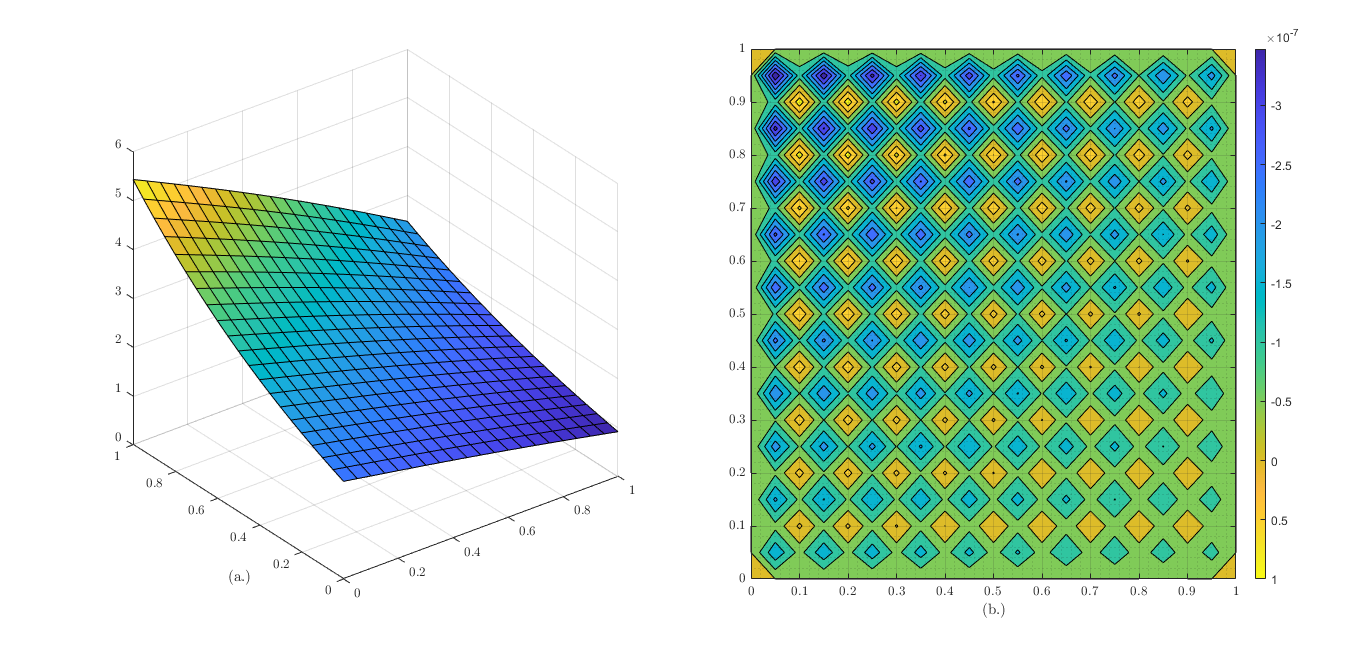
\includegraphics[scale = 0.60]{Images/poisson_comp.png}
    \caption[Approximate Solution to the Poisson Problem]{(a.) Approximate solution to the given BVP and (b.) the relative error in the analytical and the approximate solution.}
    \label{fig:Poisson_FEM}
\end{figure}
    
 The convergence of the approximate solution to the exact solution is investigated by plotting the $L^{2} error$ against
 increasing number of elements in the mesh for various Gauss quadrature points \footnote{The data for the solution with
 a singular element encompassing the domain has been skipped as it leads to a trivial solution for the case of a first
 order quardilateral element.}.

 \begin{figure}
    \centering
    \subfloat{\hspace*{-3.5cm}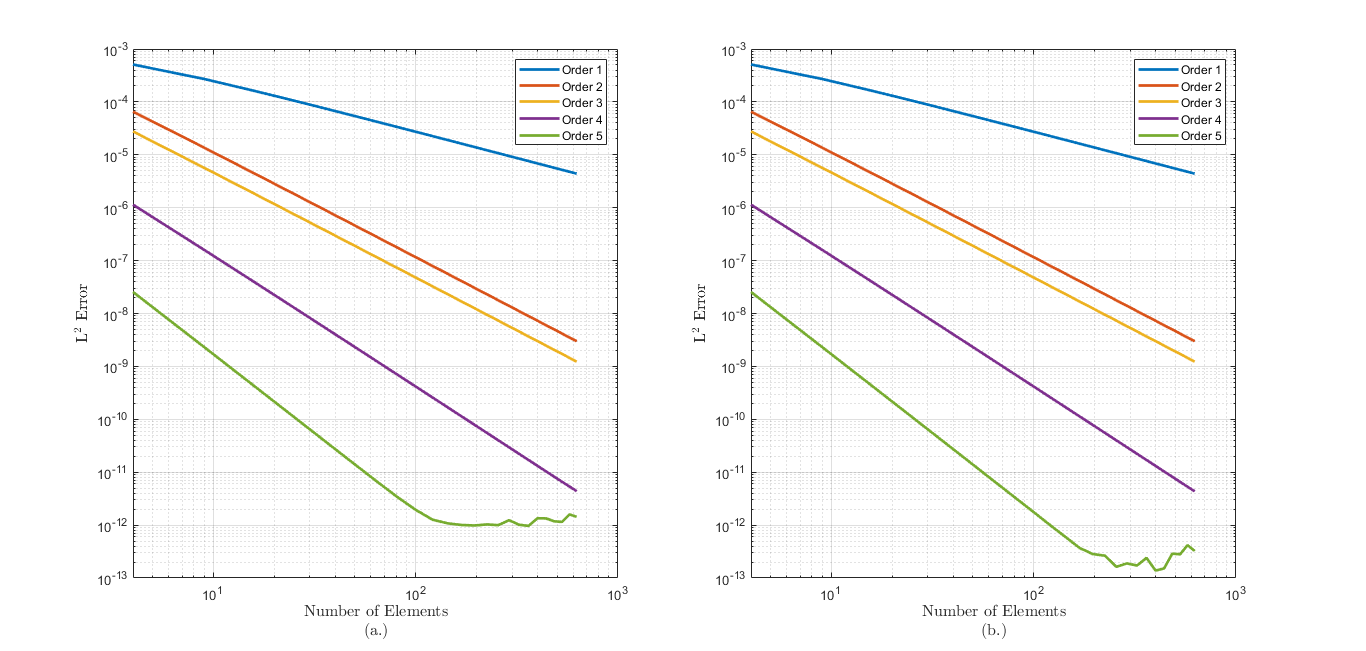
\includegraphics[scale = 0.60]{Images/conv68.png}} \\ %%\label{fig:a}} 
    \subfloat{\hspace*{-3.5cm}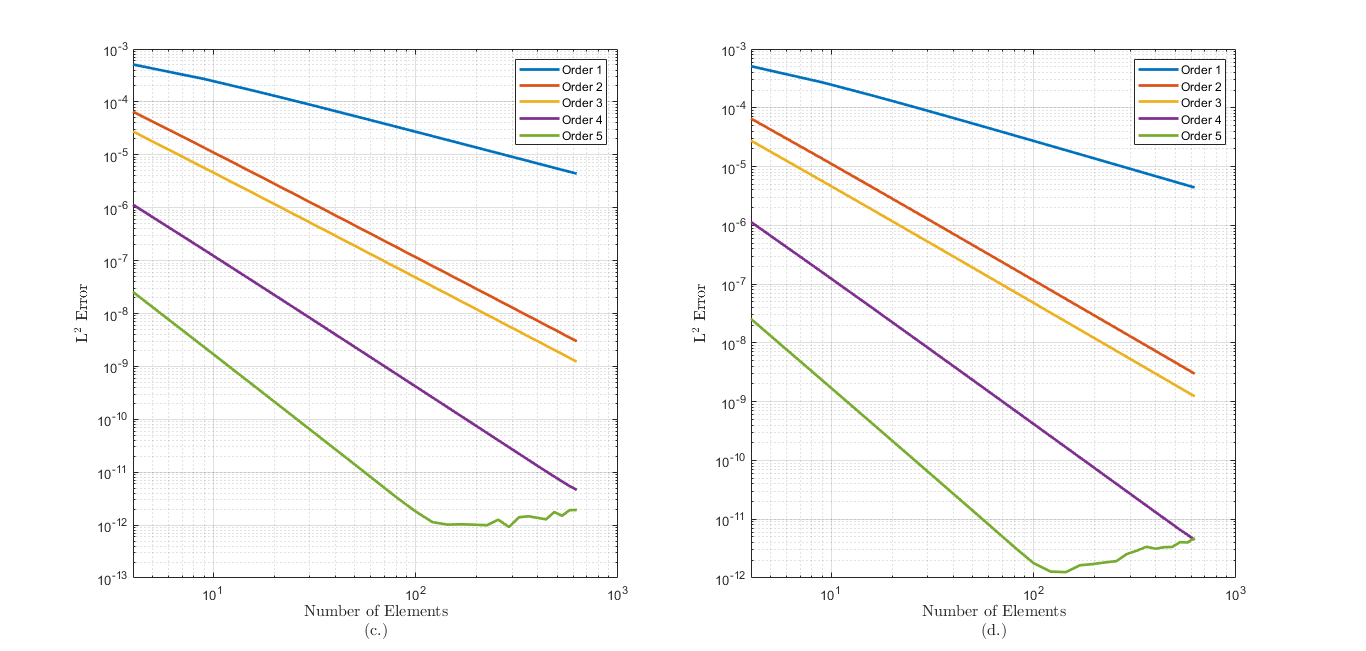
\includegraphics[scale = 0.60]{Images/conv1012.png}} %%\label{fig:b}}
    \caption[Convergence of the Approximate Solution]{Convergence of the approximate solution using various orders of approximating polynomial and (a.) 6, (b.) 8, (c.) 10, and (d.) 12 Gauss-Quadrature points.} %%\label{fig:AB}
  \end{figure}

In this section we developed the Finite Element framework for the solution of boundary value problems, investigated the
 validity of the resulting approximated solutions using \emph{a posteriori} error estimates, and tested if the approximated
 solution converges to the exact solution. This was done in order to lay the foundation for the development of a more complex
 framework in the next section in order to study the nonlinear behaviour of large deformations.

\afterpage{\blankpage}